\documentclass[12pt,letterpaper,onecolumn]{report}
\usepackage[utf8]{inputenc}
\usepackage{amsmath}
\usepackage{amsfonts}
\usepackage{amssymb}
\usepackage{amstext}
\usepackage{amsthm}
\usepackage{graphicx}
\usepackage{exscale}
\usepackage[mathscr]{eucal}
\usepackage{bm}
\usepackage{eqlist}
\usepackage[usenames, dvipsnames]{color}
\DeclareGraphicsExtensions{.pdf, .jpg}
\newcommand{\harpoon}{\overset{\rightharpoonup}}

\usepackage{esint}
\usepackage{mathtools}
\usepackage{colortbl}
\usepackage{color}
\usepackage[utf8]{inputenc}

\usepackage[left=1in,right=1in,top=1in,bottom=1in]{geometry}

\usepackage{enumitem}
\usepackage{fancyhdr}
\pagestyle{fancy}
%\fancyhf{}
\lhead{\textbf{Lecture 25}}
\chead{\textbf{ENGR 4020: Mechatronics System Design}}
\rhead{10 pts}


\begin{document}
\begin{center}
Due: Wednesday 03/25/2020 by 4 PM
\\

\end{center}
\noindent\textbf{\underline{Problem 1:}}  
 \textbf{\textit{Design Problem-2 DOF Helicopter Control by Pole Placement}} [10 pts]\\
Shown below are the free-body diagram and kinematics of the 2 DOF helicopter used in Project 1.\\
\begin{figure}[ht]
\begin{center}
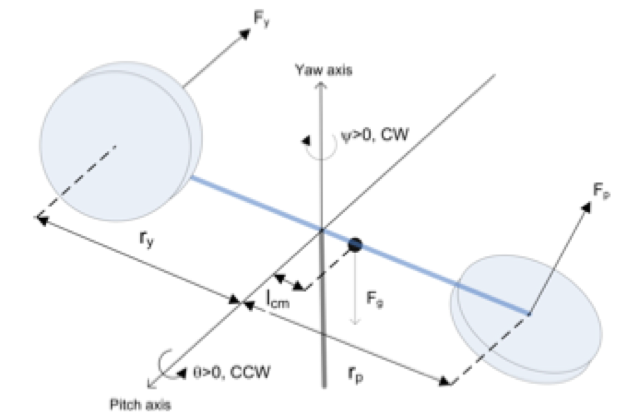
\includegraphics[width=0.5\textwidth]{Figures/helifbd.png}
\caption{2 DOF Helicopter free-body diagram.}
\end{center}
\end{figure}
\begin{figure}[ht]
\begin{center}
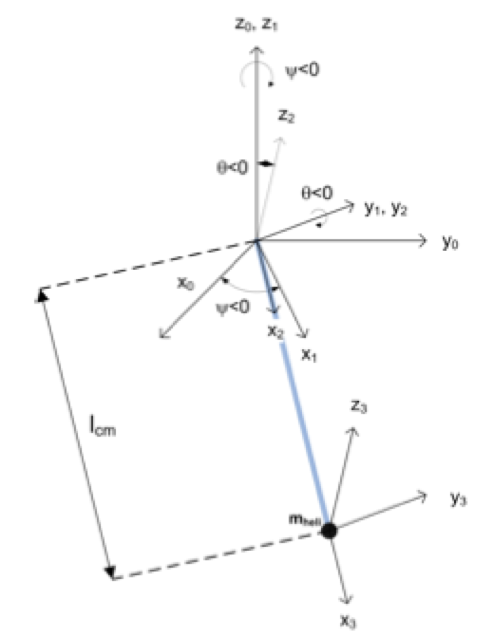
\includegraphics[width=0.40\textwidth]{Figures/helik.png}
\caption{2 DOF Helicopter kinematics diagram.}
\end{center}
\end{figure}\\
\newpage
\noindent The helicopter can be represented as a two input-two output state space model, where the state vector is defined as
$$ x=\begin{bmatrix}
\theta(t)\\\psi(t)\\\dot{\theta}(t)\\\dot{\psi}(t)
\end{bmatrix}
$$ 
and the output vector is defined as 
$$y=\begin{bmatrix}
\theta(t)\\\psi(t)
\end{bmatrix}$$
where $\theta$ is the pitch angle and $\psi$ is the yaw angle. The inputs are the commanded pitch and commanded yaw.  The state space model of this system is represented by the matrices
$$A = \begin{bmatrix}
0 & 0 & 1 & 0 \\ 0 & 0 & 0 & 1 \\ 0 & 0 & -\frac{B_p}{J_{T_p}} & 0 \\ 0 & 0 & 0 & -\frac{B_y}{J_{T_y}}
\end{bmatrix}$$
$$B = \begin{bmatrix}
0 & 0 \\ 0 & 0 \\ \frac{K_{pp}}{J_{T_p}} & \frac{K_{py}}{J_{T_p}} \\ \frac{K_{yp}}{J_{T_y}} & \frac{K_{yy}}{J_{T_y}}
\end{bmatrix}$$
$$C = \begin{bmatrix}
1 & 0 & 0 & 0 \\ 0 & 1 & 0 & 0
\end{bmatrix}$$
$$D = \begin{bmatrix}
0 & 0 \\ 0 & 0
\end{bmatrix}$$
where 
$$J_{T_p}=J_{eq\_p}+m_{heli}l_{cm}^2$$
$$J_{T_y}=J_{eq\_y}+m_{heli}l_{cm}^2$$
for the parameters in the table below.\\
\begin{table}[ht]
\begin{center}
\caption{Model parameters for the 2 DOF Helicopter}
\begin{tabular}{|c|c|c|}
\hline 
\textbf{Parameter} & \textbf{Value} & \textbf{Units and Description} \\ 
\hline 
$K_{pp}$ & 0.204 & [Nm/V] Thrust force constant on pitch axis from pitch propeller \\ 
\hline 
$K_{yy}$ & 0.072 & [Nm/V] Thrust force constant on yaw axis from yaw propeller \\ 
\hline 
$K_{py}$ & 0.0068 & [Nm/V] Thrust force constant on pitch axis from yaw propeller \\ 
\hline 
$K_{yp}$ & 0.0219 & [Nm/V] Thrust force constant on yaw axis from pitch propeller \\ 
\hline 
$B_p$ & 0.800 & [N/V] Equivalent viscous damping about pitch axis \\ 
\hline 
$B_y$ & 0.318 & [N/V] Equivalent viscous damping about yaw axis \\ 
\hline 
$m_{heli}$ & 1.3872 & [kg] Total moving mass of the helicopter \\ 
\hline 
$l_{cm}$ & 0.186 & [m] Center of mass length from pitch axis \\ 
\hline 
$J_{eq\_p}$ & 0.0384 & [kg$\cdot$m$^2$] Total moment of inertia about pitch axis \\ 
\hline 
$J_{eq\_y}$ & 0.0432 & [kg$\cdot$m$^2$] Total moment of inertia about yaw axis \\ 
\hline 
\end{tabular} 
\end{center}
\end{table}
\newpage
\noindent In this problem, you will write MATLAB code to design a controller and simulate the system response.  Start the MATLAB code with the system parameters shown in the table, and by defining the state matrices.\\
\noindent(a) Calculate the eigenvalues of the open loop system using the MATLAB command \textit{eig} [1 pt].\\
\noindent(b) Determine if the system is controllable [1 pt].\\
\noindent(c) Choose pole locations to meet the following requirements:
\begin{itemize}
\item $M_p(\%)\leq5\%$
\item $T_s<3$ s
\end{itemize}
You will want to choose the same pole locations twice so that pitch and yaw both meet the performance criteria.  In other words: \textit{p\_cl = [p\_secorder,p\_secorder]} [2 pts].\\
\noindent(d) Use the \textit{place} command to find the $K$ matrix that locates closed loop poles where you want them [1 pt].\\
\noindent(e) Collect the closed loop system using the $ss$ command, making certain to be careful with dimensions for $B$ and $D$ [1 pt].\\
\noindent(f) Find the eigenvalues of the closed loop system using the MATLAB command \textit{eig}.  Do these match the poles you chose in part (e) [1 pt]?\\
\noindent(g) In the closed loop system, the command \textit{initial} is the same as an input, as $r=-Kx$.  Find the system response by using the \textit{initial} command for an initial state of $x^T=[-10,-10,0,0]$ and a final time of 5 seconds.  This corresponds to a 10 degree step in the pitch and yaw axes.  Plot the resulting output in an appropriately labeled figure.  Note that the output will be a 2715x2 matrix, so you want to plot each column separately and label them correctly [2 pts].\\
\noindent(h) Does this output meet the requirements we set?  Can you think of some reasons why or why not [1 pt]?\\


\end{document}
